\documentclass[journal=jprobs,manuscript=article,layout=traditional]{achemso}
\usepackage[T1]{fontenc}
\usepackage[utf8]{inputenc}
\usepackage{amsmath,amssymb,booktabs,array}
\usepackage{microtype,xurl,float}
\usepackage{graphicx}
\usepackage{caption,setspace}
\captionsetup{font={small,singlespacing},justification=raggedright,singlelinecheck=false}
\usepackage[hidelinks]{hyperref}
\setkeys{acs}{articletitle=true,doi=true,maxauthors=15,etalmode=truncate}
\graphicspath{{figures/}}
\newcommand{\gene}[1]{\textit{#1}}
\newcolumntype{L}[1]{>{\raggedright\arraybackslash}p{#1}}
\emergencystretch=3em
\raggedbottom
\author{Zhiyong Tao}
\altaffiliation{Zhiyong Tao, Juan Xiong, and Yiwei Zhang contributed equally to this work.}
\author{Juan Xiong}
\altaffiliation{Zhiyong Tao, Juan Xiong, and Yiwei Zhang contributed equally to this work.}
\author{Yiwei Zhang}
\altaffiliation{Zhiyong Tao, Juan Xiong, and Yiwei Zhang contributed equally to this work.}
\author{Chulin Zhong}
\author{Wenkai Gao}
\author{Guohua Fan}
\author{Yabing Huang}
\email{ybhuang@whu.edu.cn}
\phone{+86 17625308115}
\affiliation{Department of Pathology, Renmin Hospital of Wuhan University, Wuhan 430060, China}
\title{Structure-Guided Proteogenomics Identifies ARID1A-Associated cBAF Protein Co-variation in Lung Cancer}
\keywords{ARID1A, canonical BAF, proteogenomics, protein co-variation, lung cancer, structural proteomics}
\begin{document}
\begin{abstract}
Protein co-variation can reveal complex organization, but its interpretation requires separating molecular association from selective essentiality. We asked whether six cBAF proteins selected from deposited ARID1A-contact structures show reproducible protein co-variation in lung cancer. Contact assignments persisted across two deposits, three distance thresholds, and residue-quality filtering. We compared Spearman correlations of RNA-, copy-number-, and lineage- or purity-adjusted protein residuals with a fixed six-protein BAF-family background. Differences in median correlation were 0.255 in cell lines, 0.250 in lung adenocarcinoma (108 patients; 95\% bootstrap interval 0.128--0.394; $q=0.0012$), and 0.170 in lung squamous-cell carcinoma (107 patients; 0.052--0.317; $q=0.0314$). All six selected proteins ranked among the top 28 of 7,939 eligible proteins in adenocarcinoma and within the top 5\% of 8,649 proteins in squamous carcinoma. Matched non-BAF panels, global-proteome adjustment, and influence analyses contextualized this enrichment. Published knockout proteomics showed concordant panel reductions, whereas independent fitness screens supported ARID1B more consistently than whole-panel dependence. These analyses establish reproducible co-variation of a structure-selected cBAF panel; the available background cannot isolate a direct-contact effect from shared complex membership. The study provides a bounded proteogenomic phenotype for further mechanistic investigation.
\end{abstract}

\section{Introduction}

Mammalian SWI/SNF chromatin-remodelling complexes are recurrently altered in cancer and occur as canonical BAF (cBAF), polybromo-associated BAF (PBAF) and non-canonical BAF (ncBAF) assemblies with overlapping and assembly-selective subunits \citep{kadoch2013,mashtalir2018,michel2018,wanior2021}. ARID1A is a large cBAF subunit and tumour suppressor that is altered in multiple malignancies, including non-small-cell lung cancer. Because BAF-family proteins participate in partially overlapping assemblies, a correlation between ARID1A and another BAF gene does not by itself identify physical contact, cBAF specificity or a vulnerability created by ARID1A loss.

Recent molecular studies give this problem a more precise biological frame. Patil et al. showed that the ARID1A/ARID1B intrinsically disordered region (IDR) supports condensation and partner recruitment through separable sequence features, and that disrupting these features compromises chromatin localization and cBAF activity \citep{patil2023}. Ye et al. subsequently demonstrated in H1299 and A549 lung cancer cells that co-condensation between cBAF and transcription factors, including GATA2, regulates chromatin accessibility and gene expression; deletion or sequence perturbation of the ARID1A condensation-driving IDR impaired rescue phenotypes \citep{ye2026}. These studies establish that ARID1A contributes both to stable complex organization and to dynamic, locus-selective recruitment. They also show why a genome-wide association map requires a focused molecular interpretation.

Two functional questions must remain distinct. Continuous co-dependency asks whether cell lines that require ARID1A also tend to require another gene. Loss-conditioned dependency asks whether a defined ARID1A alteration or engineered knockout increases the fitness cost of perturbing that gene. The established ARID1A--ARID1B paralogue interaction addresses the second question \citep{helming2014,ito2021,koferle2022}; a positive baseline correlation does not. Likewise, coordinated protein abundance can reflect complex membership, stoichiometry, unassembled-subunit degradation, copy-number attenuation or shared regulation, as shown in prior cancer proteogenomic studies \citep{ryan2017,goncalves2017}. It does not by itself identify a direct-contact mechanism or establish synthetic lethality.

We therefore focused this study on one testable question: does a structure-selected panel of ARID1A-contacting cBAF proteins show reproducible co-variation in lung cancer models and independent lung tumour cohorts (Figure~\ref{fig:workflow})? The fixed six-protein panel was evaluated against a measured BAF-family background and proteome-wide matched null panels. The comparison was designed to test reproducibility of the selected panel, not whether direct contact itself causes co-variation. Published ARID1A perturbation data and loss-conditioned fitness screens were analysed as biological context and boundary tests rather than interchangeable validation.

\begin{figure}[H]
\centering
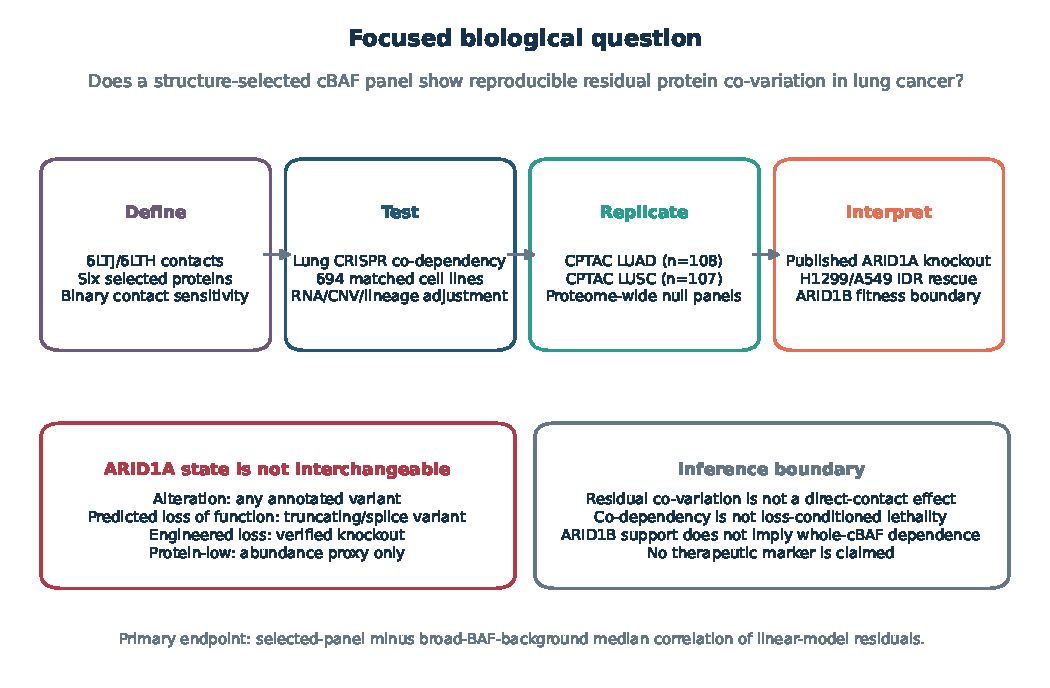
\includegraphics[width=\textwidth,height=0.60\textheight,keepaspectratio]{Figure1.pdf}
\caption{\textbf{Focused evidence chain and interpretation boundaries.} Deposited structures select a fixed six-protein cBAF panel. Genetic co-dependency supplies exploratory context; matched cell-line and tumour proteogenomes test residual protein co-variation; published knockout data provide molecular-response context. Loss-conditioned fitness is evaluated separately. Mutation, predicted loss of function, low protein abundance and engineered knockout are not treated as equivalent states. The design does not isolate direct contact from common cBAF membership.}\label{fig:workflow}
\end{figure}

\section{Experimental Section}

\subsection{Focused study design}

The primary endpoint was the difference between the median ARID1A protein correlation of six structure-selected, experimentally contacting cBAF proteins and that of six measured BAF-family background proteins after adjustment for molecular and sample covariates. The selected panel comprised SMARCC2, SMARCA4, SMARCD1, SMARCB1, SMARCE1 and DPF2. The measured background comprised ACTL6A, PBRM1, ARID2, BRD7, PHF10 and BRD9. The broad Project Score pattern was observed first and motivated structural restriction; its six-versus-eight comparison is therefore exploratory context, not an independent confirmation. The six-versus-six proteogenomic panel was frozen after assay-coverage checks and before the association scripts were run, but the study was not preregistered. LUAD and LUSC were selected for coordinated assay coverage before their panel associations were tested; the later proteome-wide and leave-one-out analyses were specified after the primary fixed-panel results and are labelled exploratory. The background is a broad BAF-family comparison rather than a set of proven noncontacts in the same cBAF particle. All analyses used public data; no new biological experiments were conducted.

Genome-scale co-dependency defined the functional-genomic context; deposited coordinates defined physical contact; matched cell-line and tumour proteogenomes tested protein coupling; published knockout proteomics tested molecular response; and independent RNAi or CRISPR screens tested loss-conditioned fitness. These endpoints were interpreted separately. Analyses not required for the focused hypothesis, including grouped machine learning, broad single-cell context, predicted interfaces and cross-complex member-removal controls, are retained in the Supplementary Information as exploratory work.

\subsection{ARID1A state definitions}

To avoid treating non-equivalent states as ``ARID1A loss'', we used the terminology in Table~\ref{tab:states}. Only source-verified engineered knockout was called knockout. Mutation, predicted loss of function and protein-low status were described by their operational definitions and were not assumed to represent biallelic functional loss.

\begin{table}[htbp]
\caption{Operational ARID1A states and permitted interpretation.}\label{tab:states}
\centering
\small
\begin{tabular}{L{0.20\textwidth}L{0.29\textwidth}L{0.39\textwidth}}
\toprule
State & Operational definition & Interpretation used in this study \\
\midrule
Any annotated mutation & Deposited mutation flag, irrespective of variant consequence & Genomic alteration; not synonymous with loss of function \\
Predicted loss of function & Nonsense, frameshift or splice-site annotation & Putative disruptive variant; not proof of biallelic loss \\
Biallelic-like proxy & Predicted loss of function plus copy number $\leq1$, or copy number zero & Sparse descriptive proxy only; no inferential claim \\
Protein-low & Bottom pre-specified fraction of measured ARID1A abundance & Abundance-defined state; not a knockout genotype \\
Engineered knockout & Source study reported targeted ARID1A knockout with molecular verification & Experimental loss in the stated cell model; not automatically generalizable to lung tumours \\
\bottomrule
\end{tabular}
\end{table}

\subsection{Genetic co-dependency}

Primary co-dependency used the de-duplicated Sanger Project Score screen (128 lung cancer models; 930 models across 19 tissues) \citep{behan2019,pacini2021}. Spearman correlations between ARID1A and all screened genes were adjusted genome-wide by the Benjamini--Hochberg (BH) procedure \citep{benjamini1995}. DepMap 24Q4 and the targeted 26Q1 update were used for release-matched sensitivity analysis on common ModelIDs. The anchor was excluded from every module score. Within-tissue estimates were computed within tissue rather than inferred from the pooled pan-cancer analysis. These analyses quantify continuous co-dependency and do not test a loss-conditioned effect.

\subsection{Experimental structures and contact robustness}

PDB 6LTJ and 6LTH were parsed with Biopython \citep{cock2009,he2020}. A contact required at least one inter-chain heavy-atom pair within 4.5\,\AA{}; chain identities were checked against deposited records. Contact counts were used only descriptively and not interpreted as a dose--response. Official wwPDB validation XML and deposited mmCIF coordinates supplied resolution, global and chain Q-scores and residue-level Q-scores. Contacts were recomputed at 4.0, 4.5 and 5.0\,\AA{} and after removal of the bottom decile of residue Q-scores within each analysed chain. The EMD-0974 panel is a projection of the deposited three-dimensional density at the depositor's contour level, not a raw particle micrograph.

For the genetic context, the six contacts were compared with eight pre-specified BAF-family comparators using exact two-sided Mann--Whitney tests, Cliff's delta and 20,000-resample percentile-bootstrap intervals (seed 20260901). SMARCC1, supported by the integrative model 9A0K rather than density-refined 6LTJ, was excluded from the fixed six-contact proteogenomic panel. Full structural prediction and mutation-mapping analyses are reported only in the Supplementary Information.

\subsection{Matched protein--RNA--copy-number analysis}

Cell-line analysis combined Sanger's averaged protein matrix dated 2025-02-11 with DepMap 24Q4 RNA, relative copy number and lineage annotations. Of 948 Sanger models, 941 mapped to Broad ModelIDs and 694 patient-distinct models had all three assays. Protein values were retained on the provided normalized scale, RNA as $\log_2(\mathrm{TPM}+1)$ and relative copy number as $\log_2(\mathrm{CN}+1)$. No missing protein values were imputed.

For each partner, protein abundance was regressed on its own RNA, own copy number and lineage; the reported estimand was the Spearman correlation between its ordinary-least-squares residuals and equivalently adjusted ARID1A protein residuals. This is a rank correlation of linear-model residuals, not a general covariate-adjusted Spearman coefficient under arbitrary nonlinear effects. Each pair used identical complete-case rows and required at least 40 observations and 20 residual degrees of freedom. The primary statistic was the median selected-panel correlation minus the median background correlation. A lineage-stratified shared-row bootstrap (10,000 draws, seed 20260904) refitted all regressions in every draw. We report percentile intervals and two-sided centred-bootstrap approximate probabilities, with BH correction across the two discovery endpoints.

External tests used the coordinated CPTAC pan-cancer data freeze v1.2, with LUAD and LUSC analysed separately \citep{li2023proteogenomic,gillette2020,satpathy2021}. Exact GENCODE-v34 mappings aligned reference-normalized protein, upper-quartile-normalized RNA and WES copy-number values. One tumour sample per patient was retained. Excluding one case with missing WES-derived purity from each cohort left 108 LUAD and 107 LUSC patients. Purity replaced lineage in the regression, and the same 10,000-draw shared-row bootstrap was applied independently by cohort. The four external tests comprised two cohort-specific selected-panel-minus-background residual-correlation contrasts and two cohort-specific raw protein-minus-RNA contrasts; BH correction covered this four-test family. Cohorts were not pooled.

\subsection{Proteome-wide specificity and sensitivity analyses}

The fixed-panel model was extended to every complete-case protein with finite and variable protein, RNA and copy-number measurements in each CPTAC cohort, excluding ARID1A. The six-contact median was compared with 20,000 size-six non-BAF panels under two competitive nulls: uniform size-matched sampling and matching to each contact's nearest non-BAF proteins in mean protein, protein variability, mean RNA and RNA variability. The one-sided Monte Carlo probability used a plus-one correction, and BH adjustment covered four cohort-by-null comparisons. These gene-set comparisons do not create additional patient cohorts.

Sensitivity analyses added the first 1, 3 or 5 principal components of standardized, own-adjusted residual proteins after excluding BAF-family genes. Each patient was also omitted once and the base model refitted. Leave-one-subunit-out estimates assessed dependence on any single member of the 12-protein fixed panel. These analyses were specified after the primary fixed-panel results and are therefore labelled exploratory.

\subsection{Published molecular perturbation data}

The original Table S6 from Roumeliotis et al. was used to extract the unchanged panel in induced pluripotent stem cells \citep{roumeliotis2017}. For ARID1A, ARID2 and PBRM1 knockout conditions, descriptive protein change was $\log_2[\mathrm{mean(KO)}/\mathrm{mean(WT)}]$ from the author-scaled TMT values, with two labelled clones per condition. Source RNA log-fold changes and DESeq2-adjusted probabilities were retained. Protein omnibus probabilities across all four conditions were not reinterpreted as knockout-versus-WT tests, and no new protein significance test was asserted.

To contextualize the molecular phenotype, we integrated two independent experimental studies \citep{patil2023,ye2026}. Patil et al. supplied evidence that the ARID1A/B IDR controls condensation and partner recruitment. From the openly supplied source data of Ye et al., we descriptively replotted 96-hour rescue measurements from H1299 and A549 ARID1A-knockout cells for full-length ARID1A, an IDR-deletion construct and a tyrosine-to-alanine IDR mutant, with or without GATA2 (five source observations per condition). Means and standard deviations were calculated directly from the deposited values. We introduced no new statistical test and did not treat these published observations as a new independent experiment performed by the present authors.

\subsection{Loss-conditioned fitness as a boundary analysis}

Project DRIVE deep-RNAi data included 354 usable models across 17 lineages \citep{mcdonald2017,srivatsa2022}. Genes were standardized within lineage. Any annotated mutation and predicted loss-of-function states followed Table~\ref{tab:states}; a biallelic-like proxy contained only four models and was descriptive. ARID1B and pre-specified BAF modules were compared between state groups by two-sided Mann--Whitney tests with BH correction within each state definition and 20,000-resample intervals. ARID1B robustness was checked by leave-one-lineage-out analysis.

Published 14-day U2-OS and RMG-1 and 21-day 293A screens were analysed on their source gene-level scales \citep{awwad2025,fournier2024,feng2022}. The 293A model retained an ARID1A protein species and was not called a complete knockout. The HAP1 ARID1A-query interaction matrix was analysed with exhaustive fixed-panel gene-label permutations; the source used one knockout clone with technical endpoints \citep{billmann2026}. These resources test context-specific fitness, not the patient protein-coupling endpoint.

\subsection{Statistical reporting and reproducibility}

Cell lines, source patients, genes and published experimental observations were treated as distinct units. Resampling unit, correction family, test direction and random seed are specified above and in the Supplementary Information. Confidence intervals are nominal unless stated otherwise. Non-significance was not interpreted as equivalence. Scripts, source identifiers, checksums, sample attrition and complete derived tables are supplied in Supplementary Data S1--S8. All numeric results were generated from archived inputs by the supplied scripts.

\subsection{Ethics and source-data governance}
This study re-analysed previously published, de-identified public datasets and deposited molecular structures. No participants were recruited and no new human or animal experiments were performed. Original consent and ethics procedures are described in the source publications. No re-identification was attempted. Original raw proteomic accessions and the distinction between source data and derived outputs are provided under Data and Code Availability.

\section{Results}

\subsection{Experimental structures select a fixed six-protein cBAF panel}

Seven SWI/SNF genes occurred among the ten highest-ranked ARID1A co-dependencies in the 128-model lung Project Score analysis, motivating a structure-based restriction of the candidate set (Figure~\ref{fig:workflow}). Deposited cBAF coordinates identified six proteins with direct ARID1A heavy-atom contacts: SMARCC2, SMARCA4, SMARCD1, SMARCB1, SMARCE1 and DPF2 (Figure~\ref{fig:structure_focused}). These proteins form the fixed, structure-selected panel used in every primary proteogenomic test.

The binary assignments were stable to structural uncertainty. All six contacts were retained in both 6LTJ and 6LTH at 4.0, 4.5 and 5.0\,\AA{}, and after removing residues in the bottom Q-score decile. The 6LTJ global Q-score was low (0.007), whereas the related base-module deposit 6LTH had a global Q-score of 0.526; the agreement of binary calls across deposits and filters therefore supports panel membership, but not atomically precise mechanistic claims from 6LTJ alone. In exploratory genetic comparisons, the structure-selected proteins had higher ARID1A co-dependency than eight broad BAF-family comparators: the difference in median correlation was 0.432 in lung models (95\% bootstrap interval 0.162--0.590; Cliff's $\delta=0.833$; exact $P=0.0080$) and 0.279 pan-cancer (0.090--0.471; $\delta=0.792$; $P=0.0127$). Because the broad co-dependency pattern motivated panel selection, these are descriptive context rather than independent confirmation. The smaller same-deposit six-versus-two comparison was unsupported ($P=0.286$ in both cohorts), so current data do not isolate direct contact from shared cBAF membership. Contact count itself was not interpreted as a graded predictor.

\begin{figure}[H]
\centering
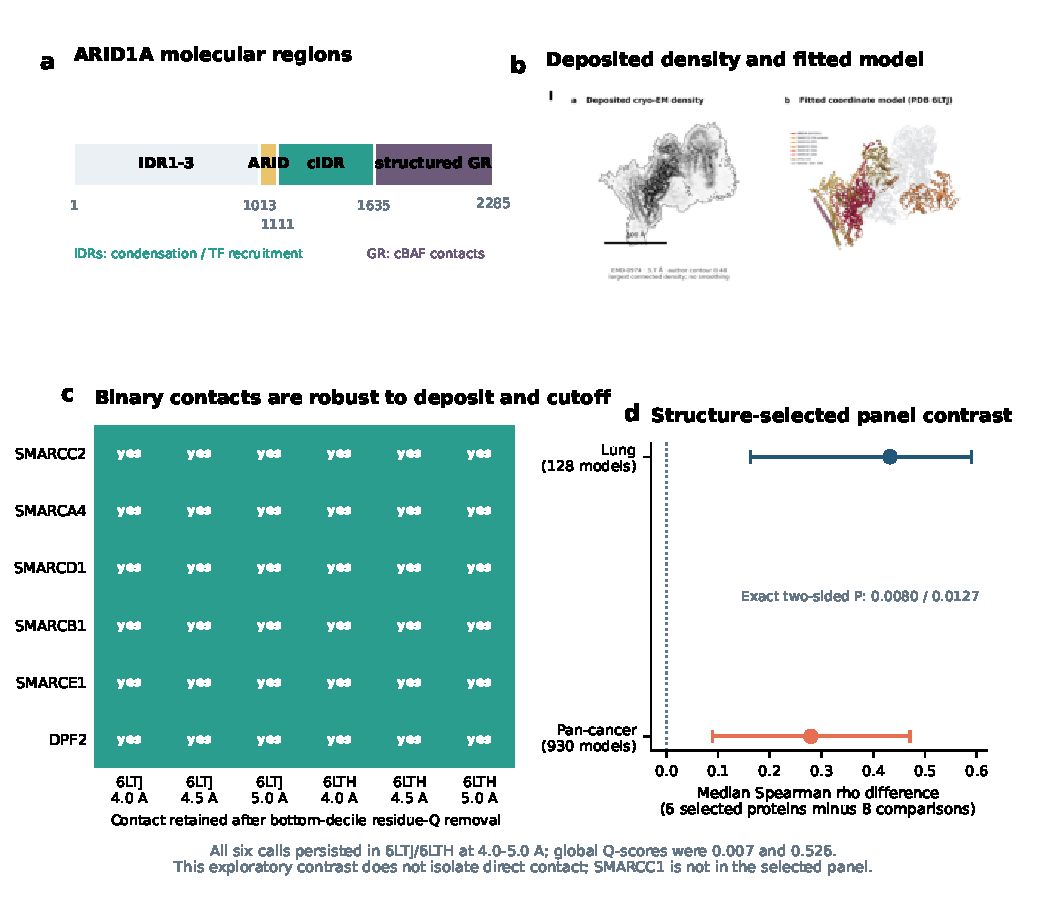
\includegraphics[width=\textwidth,height=0.60\textheight,keepaspectratio]{Figure2.pdf}
\caption{\textbf{Experimental structures select a robust six-protein cBAF panel.} (\textbf{a}) ARID1A domain architecture distinguishes the condensation-driving intrinsically disordered region (cIDR) from the ordered C-terminal region represented in deposited structures. (\textbf{b}) Grayscale projection of deposited EMD-0974 density and fitted PDB 6LTJ model; the density is not a raw micrograph. (\textbf{c}) All six contacts are retained in 6LTJ and 6LTH at 4.0, 4.5 and 5.0\,\AA{} and after removal of locally low-Q residues. Global Q-scores caution against atomically precise interpretation of 6LTJ. (\textbf{d}) Exploratory six-versus-eight BAF-family co-dependency contrasts; points are differences in median Spearman correlation and bars are 95\% percentile-bootstrap intervals. Exact two-sided Mann--Whitney probabilities are shown. Panel selection was motivated by the broad co-dependency pattern, so this is not independent confirmation. Contact count is not interpreted as a dose--response; SMARCC1 is not included in the selected six-protein panel.}\label{fig:structure_focused}
\end{figure}

\subsection{The structure-selected panel shows reproducible residual protein co-variation}

In 694 patient-distinct pan-cancer cell lines, Spearman correlations between linear-model residuals were higher for the six structure-selected proteins than for the six BAF-family background proteins after adjustment for each partner's RNA, copy number and lineage (Figure~\ref{fig:coupling}). The selected-panel-minus-background difference in median correlation was 0.255 and remained positive under common-covariate and leave-one-lineage sensitivities. This result measures residual protein co-variation under a linear, additive adjustment model; it is not a physical-complex occupancy fraction or proof that direct contact causes the contrast.

The same fixed analysis replicated in two independent lung-tumour cohorts. After adjustment for each partner's RNA, copy number and tumour purity, the median difference was 0.250 in LUAD (108 patients; 95\% interval 0.128--0.394; $q=0.0012$) and 0.170 in LUSC (107 patients; 0.052--0.317; $q=0.0314$). Removing any one subunit retained a positive estimate in both cohorts (LUAD 0.218--0.283; LUSC 0.167--0.174). The LUAD-minus-LUSC difference was 0.080 (95\% interval $-0.105$ to 0.265; $P=0.407$), which neither establishes a histology difference nor equivalence. Four background proteins also showed positive co-variation in both cohorts, so the result is relative enrichment of the selected panel rather than exclusive cBAF specificity.

Raw protein-over-RNA separation was supported in cell lines but not in either tumour cohort. We therefore do not claim that protein-level coordination is universally stronger than transcriptional coordination. Instead, the replicated result is the linear-model-residual contrast between a structure-selected panel and the fixed BAF-family background.

\begin{figure}[H]
\centering
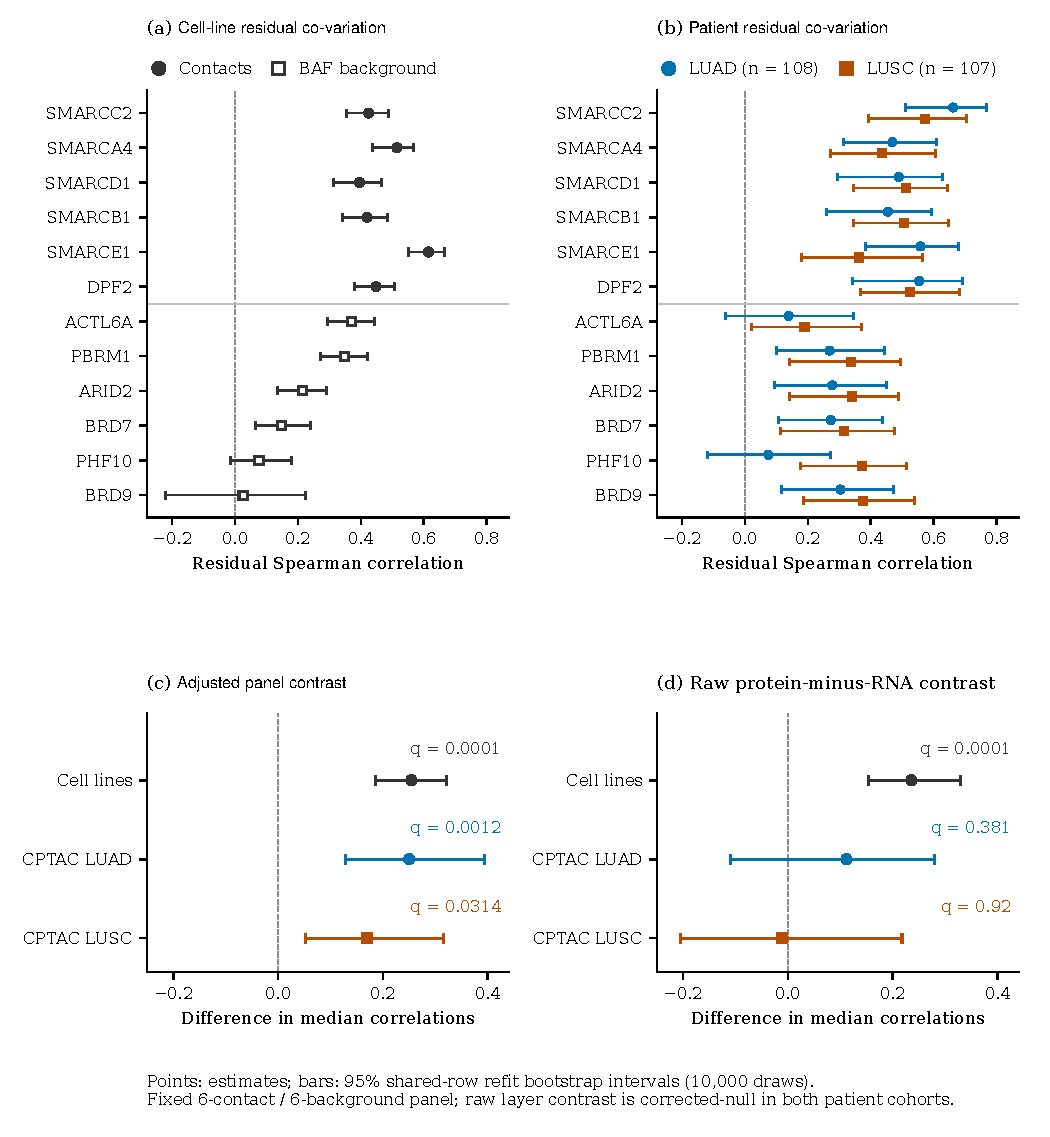
\includegraphics[width=\textwidth,height=0.60\textheight,keepaspectratio]{Figure3.pdf}
\caption{\textbf{Residual protein co-variation replicates in lung tumours.} (\textbf{a}) Spearman correlation between linear-model residuals of ARID1A and six structure-selected or six BAF-family background proteins in 694 patient-distinct cell lines; each protein was adjusted for its own RNA, copy number and lineage. (\textbf{b}) The same analysis in CPTAC LUAD (108 patients) and LUSC (107 patients), with WES-derived purity replacing lineage. (\textbf{c}) Selected-panel-minus-background difference in median residual correlation. (\textbf{d}) Raw protein-minus-RNA contrast on the same rows; neither patient-cohort contrast received corrected support. Bars are 95\% percentile intervals from 10,000 shared-row bootstrap draws with regressions refitted. Missingness was not imputed. The background contains mutually exclusive BAF subunits rather than sufficient same-particle noncontacts; the contrast does not isolate a direct-contact effect, complex occupancy or patient dependency.}\label{fig:coupling}
\end{figure}

\subsection{Proteome-wide controls and knockout proteomics localize the phenotype}

The complete-case scan included 7,939 proteins in LUAD and 8,649 in LUSC (Figure~\ref{fig:proteome}). All six selected proteins ranked among the first 28 proteins in LUAD; in LUSC they ranked 22nd--410th, all within the top 5\%. Their median residual correlations were 0.522 and 0.510, compared with 0.031 and 0.041 for expression- and variability-matched non-BAF null panels. None of 20,000 sampled panels under either null reached the selected-panel statistic in either cohort; with the plus-one correction, all four BH-adjusted probabilities were $1/20001$ ($\approx0.000050$). This value is the simulation resolution, not evidence for a smaller probability. These non-BAF nulls control expression and variability, not common protein-complex membership.

The selected-panel-minus-BAF-background contrast remained positive after adjustment for 1, 3 or 5 global residual-proteome components (LUAD 0.220--0.266; LUSC 0.106--0.239) and after omitting each patient in turn. Global components can contain biological as well as technical variation, so these are sensitivity analyses rather than a replacement primary model.

Published ARID1A-knockout iPSC data supplied a separate molecular-response endpoint \citep{roumeliotis2017}. All six selected proteins decreased at the protein level; their median protein log$_2$ fold change was $-0.468$, compared with $-0.059$ for the background. The selected-panel median RNA change was $-0.026$, and none of the six source RNA adjusted probabilities was below 0.05. Lack of RNA significance is not proof of no transcriptional response, and the two labelled protein clones per condition do not support a new gene-level significance claim. The re-analysis is consistent with a previously reported molecular response but is not independent lung-cancer or mechanistic validation.

\begin{figure}[H]
\centering
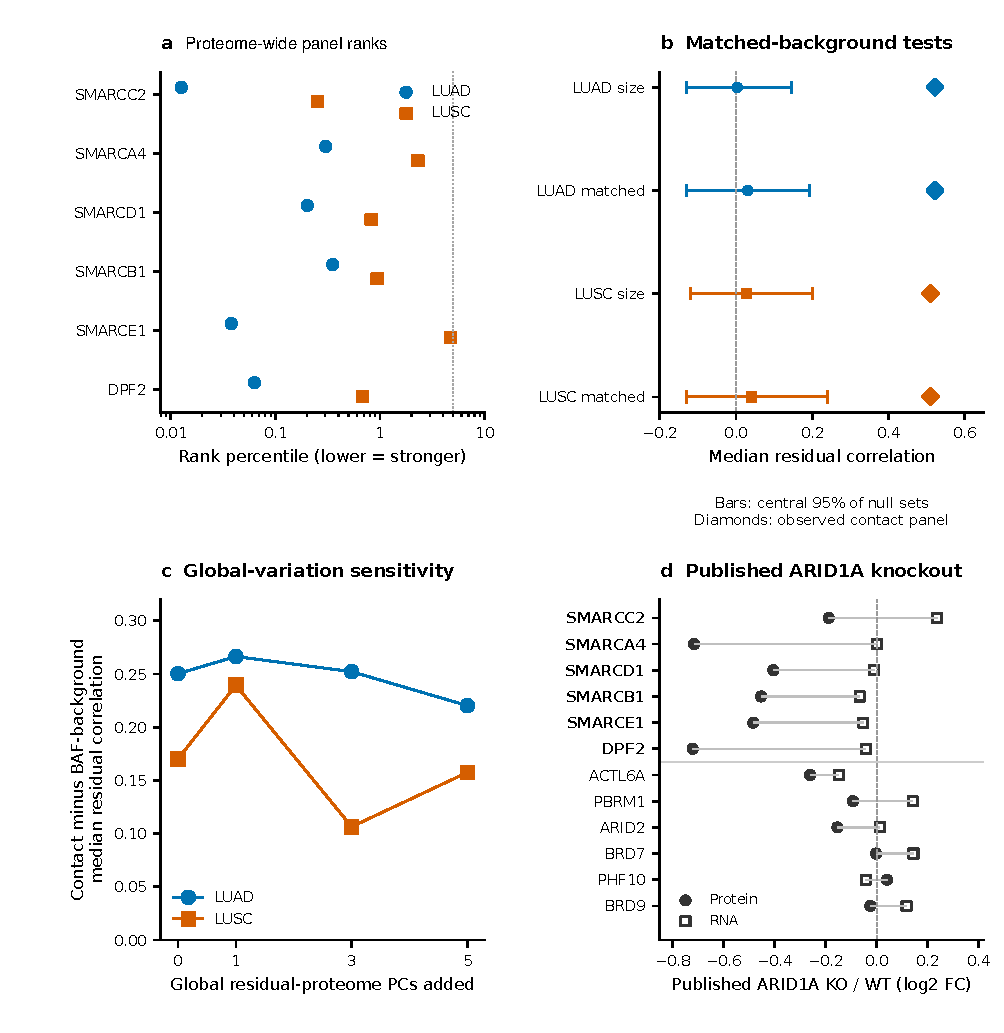
\includegraphics[width=\textwidth,height=0.60\textheight,keepaspectratio]{Figure4.pdf}
\caption{\textbf{Proteome-wide specificity and published knockout protein responses.} (\textbf{a}) Residual-correlation rank percentiles of the six selected proteins in complete-case LUAD and LUSC proteomes. (\textbf{b}) Median and central 95\% range of 20,000 non-BAF null-panel statistics under size-only and expression/variability-matched sampling; diamonds show the selected panel. These nulls do not match protein-complex membership. (\textbf{c}) Panel contrast after adjustment for 0, 1, 3 or 5 global residual-proteome components. (\textbf{d}) Published ARID1A-knockout iPSC protein changes and source RNA changes \citep{roumeliotis2017}. Protein values use two labelled knockout and two wild-type clones; RNA coefficients derive from the source RNA-seq analysis. No new protein significance test is asserted.}\label{fig:proteome}
\end{figure}

\subsection{Loss-conditioned fitness supports ARID1B, not a whole selected panel}

Independent fitness resources did not justify converting protein coupling into a therapeutic-dependency claim. In Project DRIVE, ARID1B dependency was stronger in models with any annotated ARID1A mutation (standardized difference $-0.765$, 95\% interval $-1.122$ to $-0.433$; $q=1.51\times10^{-4}$) and with predicted loss-of-function variants ($-0.844$, $-1.283$ to $-0.431$; $q=0.00152$). Every leave-one-lineage-out estimate retained the direction. In contrast, the cBAF-associated module did not survive correction ($q=0.093$ and 0.139), and coverage was incomplete.

Published isogenic screens were context-dependent. U2-OS and RMG-1 results supported gene-set signals after within-screen analysis, but direct comparisons with PBAF or ncBAF remained unsupported. The fully covered HAP1 matrix reproduced a strong ARID1B negative interaction (source qGI $=-1.724$, FDR $=4.85\times10^{-12}$), whereas contact-versus-background and cBAF-versus-PBAF/ncBAF panel comparisons were unsupported after Holm correction (all adjusted $P=0.5864$). These findings support the known paralogue dependency but do not establish module-wide or lung-specific synthetic lethality.

\section{Discussion}

This focused analysis identifies reproducible protein co-variation for a structure-selected cBAF panel around ARID1A in lung cancer. The six selected proteins showed stronger linear-model-residual correlations with ARID1A than a broad BAF-family background in cell lines and two independent tumour cohorts, occupied extreme proteome-wide ranks and decreased concordantly in a published ARID1A-knockout proteomic experiment. The strongest new evidence is therefore not another genome-scale network or a direct-contact mechanism, but replication of a fixed structural selection in patient proteogenomes under measured RNA, copy-number and purity adjustment.

The molecular literature provides context without serving as validation of this observational endpoint. The ordered C-terminal region of ARID1A provides extensive physical contacts within cBAF, whereas the IDR controls condensation and recruitment of regulatory partners \citep{patil2023,ye2026}. A descriptive replot of the Ye et al. H1299/A549 source data is retained as Supplementary Figure S20. Those experiments establish IDR-dependent behaviour in defined cell systems; the present residual-correlation analysis neither retests that mechanism nor distinguishes direct contact from common cBAF membership.

Several alternatives were tested. Stronger selected-panel co-variation was not explained by expression level or variability in matched non-BAF nulls, persisted after removal of global residual-proteome components and did not depend on any single patient or panel member. At the same time, positive co-variation of several background BAF proteins shows that the phenotype is not exclusive to the six selected proteins. The background contains proteins from mutually exclusive BAF assemblies and is not a valid same-particle noncontact set; the only smaller same-deposit comparison was underpowered and unsupported. The result should therefore be described as reproducible co-variation of a structure-selected cBAF panel, not contact-specific enrichment or a biochemical definition of cBAF.

The study also establishes an important negative boundary. Continuous co-dependency, coordinated protein abundance and loss-conditioned fitness are different endpoints. Project DRIVE and HAP1 consistently reproduced ARID1B dependence after ARID1A alteration or knockout, but did not support an entire cBAF or structure-selected panel after correction. This does not prove absence of context-specific dependencies; the public resources differ in lineage, perturbation, duration and panel coverage. It precludes presenting the panel as a validated therapeutic target set.

Limitations remain. All new analyses are computational re-analyses of public data, and no experiment was performed by the present authors. Correlations of ordinary-least-squares residuals assume linear, additive covariate effects; nonlinear and heteroscedastic effects were not comprehensively modelled. Residual protein correlations can also reflect unmeasured regulation, cell composition or technical effects. Complete-case proteome scans favour well-measured proteins. Expression- and variability-matched non-BAF nulls do not control common complex membership. The low global Q-score of 6LTJ limits atomic interpretation, although binary contact calls were robust in 6LTH and to residue-quality filtering. The iPSC experiment has two labelled protein clones per condition and is not malignant lung epithelium. The Ye et al. replot is descriptive reuse of published source data, not independent validation. Mutation and protein-low categories do not prove biallelic functional loss, and current isogenic fitness resources are not replicated protein-null NSCLC panels.

Prospective validation should therefore use multiple molecularly verified ARID1A-null NSCLC clones, full-length and domain-specific rescue, quantitative complex proteomics and longitudinal competitive fitness. Same-particle noncontact controls or a multi-complex benchmark would be required to test whether direct contact adds information beyond complex membership. The present results provide effect sizes, a reproducible panel definition and negative boundaries for that work.

\section{Conclusions}

A structure-selected panel of six ARID1A-contacting cBAF proteins shows reproducible residual protein co-variation across cancer cell lines and in two independent lung-tumour proteogenomes. The design does not isolate a direct-contact effect from common cBAF membership. Independent fitness screens support ARID1B dependence but not a whole-panel therapeutic vulnerability. The study therefore advances one bounded observational conclusion rather than a general mechanism for the cBAF system.


\begin{suppinfo}
Operational BAF definitions, structural-quality and co-dependency sensitivities, expression context, loss-conditioned fitness, proteogenomic robustness, and extended methods (PDF); grouped prediction, matched-null, and HAP1 interaction analyses (Data S1, ZIP); genetic, structural, and sustained-fitness source tables (Data S2, three ZIP parts); matched protein/RNA/copy-number inputs, analysis scripts, and bootstrap outputs (Data S3, three ZIP parts); frozen structural-prediction inputs and interface mapping (Data S4, three ZIP parts); cross-histology and subunit-influence results (Data S5, ZIP); proteome-wide ranks, matched-null panels, global-component sensitivities, and replay inputs (Data S6, two ZIP parts); published iPSC knockout protein/RNA extraction and audit (Data S7, ZIP); figure-source mapping, plotted source values, TOC artwork code, reference metadata audit, and reproducibility instructions for the present version (Data S8, ZIP).
\end{suppinfo}

\section*{Data and Code Availability}
This study reanalyzed public data and generated no new mass-spectrometry acquisition files. Original CPTAC discovery proteomes are available from the NCI Proteomic Data Commons under PDC000153 (LUAD) and PDC000232 (LUSC); the coordinated processed matrices used here are from CPTAC pan-cancer data freeze v1.2, as specified in the source manifest. Original Roumeliotis et al. proteomics are available under ProteomeXchange PXD005235; the present iPSC reanalysis used the published Table S6. Other cell-line, screening, structure, and source-table identifiers and access conditions are documented in Supporting Data S1--S8. Source raw data remain with their original repositories and licenses. No controlled-access individual genomic files are redistributed.

Analysis code, machine-readable derived results, source identifiers, checksums, and execution instructions for this version are deposited at \url{https://github.com/ArleneHarrison/arid1a-baf-collateral-dependency}, release v1.1.1, and in Zenodo under the version-specific DOI \url{https://doi.org/10.5281/zenodo.23587002}.\citep{projectcode,projectarchive} Supporting Data S1--S8 accompany the article and are included in that archive. Earlier project releases represent earlier analyses and should not be substituted for this version.

\section*{Author Information}
\subsection*{Corresponding Author}
Yabing Huang --- Department of Pathology, Renmin Hospital of Wuhan University, Wuhan 430060, China; email: \href{mailto:ybhuang@whu.edu.cn}{ybhuang@whu.edu.cn}; telephone: +86 17625308115.

\subsection*{Author Contributions}
Z.T.: conceptualization, methodology, software, formal analysis, investigation, visualization, and writing of the original draft. J.X.: methodology, formal analysis, validation, data curation, investigation, and writing of the original draft. Y.Z.: methodology, software, formal analysis, validation, data curation, visualization, and writing of the original draft. C.Z.: data curation, formal analysis, validation, and visualization. W.G.: data curation, investigation, validation, and review and editing. G.F.: conceptualization, supervision, project administration, resources, and review and editing. Y.H.: conceptualization, supervision, funding acquisition, project administration, interpretation, and review and editing. Zhiyong Tao, Juan Xiong, and Yiwei Zhang contributed equally. All authors have approved submission of the work.

\subsection*{Notes}
The authors declare no competing financial interest.

\begin{acknowledgement}
This work was supported by the General Program of the National Natural Science Foundation of China (Grant No. 62572360). We acknowledge the investigators, participants, and public resources of the original studies. During the September--October 2026 revisions, OpenAI Codex assisted with code drafting, manuscript editing, and preparation of plotting code. Numerical observations were taken from archived source data and computed by the supplied analysis scripts. Figures and the TOC graphic were rendered with deterministic plotting software; no generative image model was used. The authors are responsible for the submitted content.
\end{acknowledgement}

\bibliography{references_jpr}

\begin{tocentry}
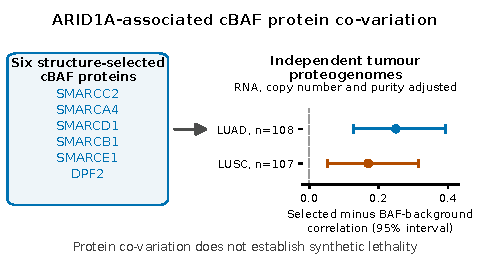
\includegraphics[width=3.25in,height=1.75in]{TOC_graphic.pdf}
\end{tocentry}
\end{document}
